\section{実験セットアップ}
図\ref{fig:ELPHSetup}に実験セットアップの概略図を示す。
$\SI{0.8}{GeV/c}$の陽電子をビームとして用いた。
T1、T2はトリガー検出器として使用したプラスチック・シンチレーターで、どちらも$\SI{10}{mm}\times\SI{10}{mm}\times\SI{5}{mm}$である。
輻射体として表\ref{table:Aerogel}に示す3つのエアロゲルを並べて使用した。
エアロゲルの中心から$\SI{1500}{mm}$離したところに九面鏡を設置し、ビームに対して$\ang{21.4}$傾けた方向に$\SI{1500}{mm}$離して設置した。
鏡はエアロゲルを設置する場所にレーザーを置き、鉛直・水平方向の光が鏡の中心にあたり検出面の中心に反射するようにアライメントを行った。
また、T1以外はチェレンコフ光以外を遮断するために遮光シートで覆った。

\begin{table}[htbp]
  \caption{使用したエアロゲルのパラメータ}
  \label{table:Aerogel}
  \centering
  \begin{tabular}{cccc}
    \hline
    型番      & 屈折率    & 厚さ (mm) & 波長400 nmに対する透過長 (mm) \\
    \hline\hline
    TSA9-3  & 1.0400 & 20.7    & 54                   \\
    TSA10-3 & 1.0395 & 10.8    & 55                   \\
    TSA9-4  & 1.0397 & 21.0    & 58                   \\
    \hline
  \end{tabular}
\end{table}


\begin{figure}
  \centering
  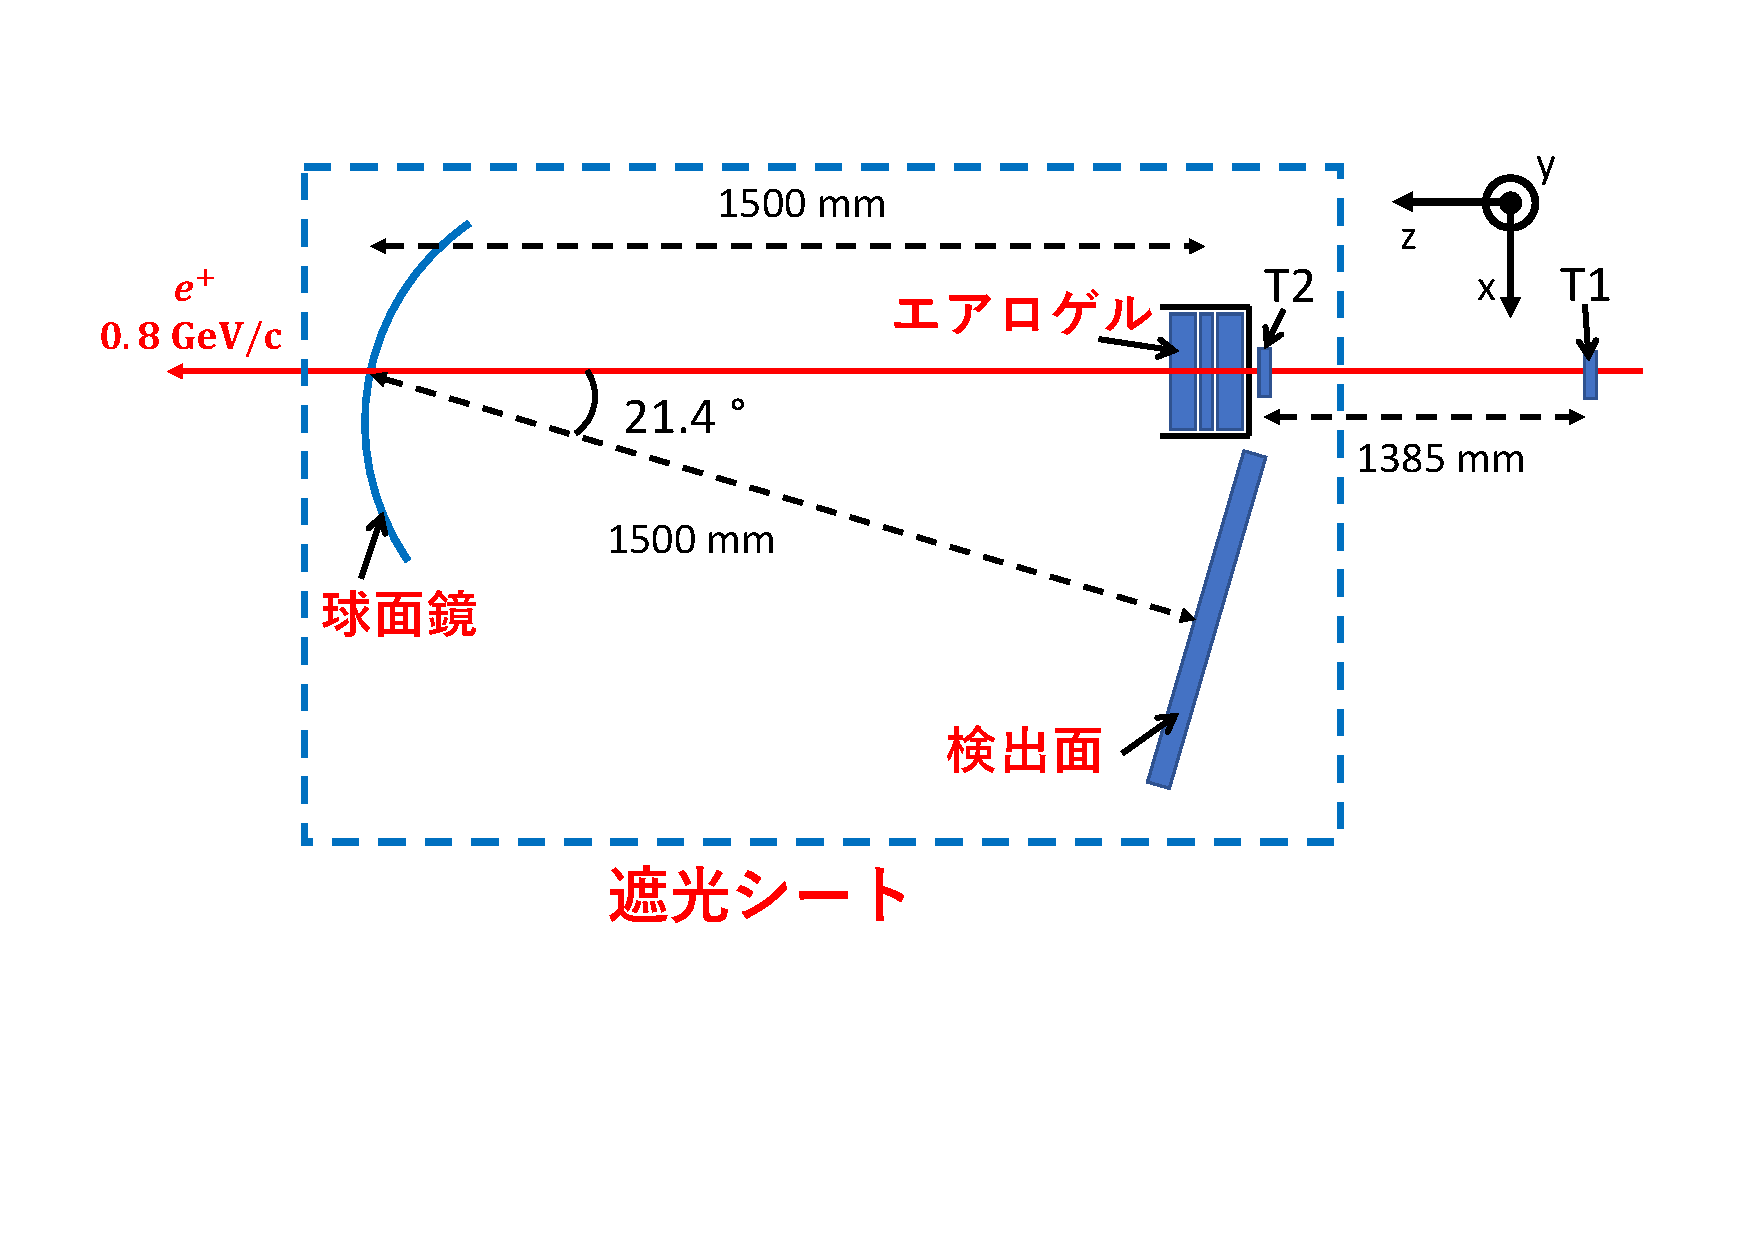
\includegraphics[width=15cm]{images/chapter3/ELPHSetup.pdf}
  \caption{実験セットアップを上から見た場合の概略図。}
  \label{fig:ELPHSetup}
\end{figure}